\section{Introduction and Problem Understanding}

\subsection{Context and Background}
The ``Plant Seedlings Classification'' challenge, hosted on Kaggle~\cite{plant-seedlings-classification}, presents a real-world problem central to modern agriculture: accurately identifying the species of young seedlings from digital images~\cite{MESHRAM2021100010}.

The dataset described in the paper ``A Public Image Database for Benchmark of Plant Seedling Classification Algorithms''~\cite{DBLP:journals/corr/abs-1711-05458} contains images of approximately \textit{960} unique plants, representing \textit{12} different species. Each image captures a seedling at different growth stages and under different conditions, reflecting the complexities found in real-world agricultural environments. These conditions include differences in lighting, background soil patterns and subtle phenotypic variations that can blur the lines between certain species. The evaluation metric of the competition is a mean~(micro-averaged) F1-score, which encourages balanced performance across classes~\cite{plant-seedlings-classification-evaluation}:

\begin{equation}
    \text{Precision}_{\text{micro}} = \frac{\sum_{k \in C} TP_k}{\sum_{k \in C} TP_k + FP_k}\label{eq:precision}
\end{equation}

\begin{equation}
    \text{Recall}_{\text{micro}} = \frac{\sum_{k \in C} TP_k}{\sum_{k \in C} TP_k + FN_k}\label{eq:recall}
\end{equation}

\begin{equation}
    F1_{\text{micro}} = \frac{2 \cdot \text{Precision}_{\text{micro}} \cdot \text{Recall}_{\text{micro}}}{\text{Precision}_{\text{micro}} + \text{Recall}_{\text{micro}}}\label{eq:fscore}
\end{equation}

where $TP_k$, $FP_k$ and $FN_k$ are the true positive, false positive and false negative counts for class $k$, respectively and $C$ is the set of all classes. The mean F1-score~(\ref{eq:fscore}) is a balanced measure that considers both precision~(\ref{eq:precision}) and recall~(\ref{eq:recall}) across all classes, making it a suitable evaluation metric for multi-class classification tasks.

\subsection{Problem Definition and Objectives}
The core objective of the challenge is to build an automated classification model that can take a seedling image as input and accurately predict its species. The following points summarize the task:

\begin{enumerate}
    \item \textbf{Input:} Test set of \textit{794} images of plant seedlings.
    \item \textbf{Output:} Classification label for each image, indicating the species of each plant seedling.
    \item \textbf{Goal:} High classification performance as measured by equation~\ref{eq:fscore}.
\end{enumerate}

\subsection{Dataset Overview}
For a better understanding of the dataset, a brief overview of the class distribution and sample images is provided below:

\begin{figure}[htbp]
    \centerline{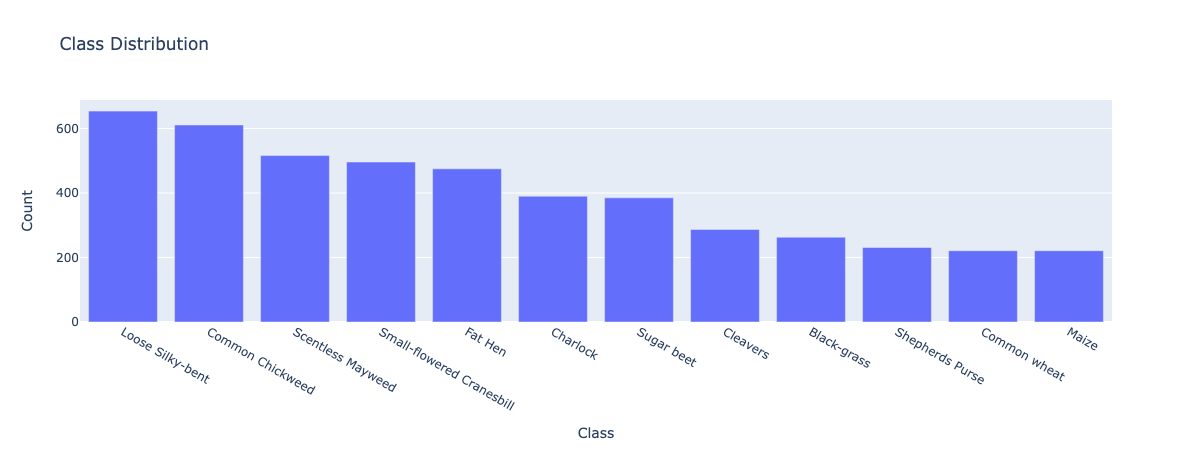
\includegraphics[width=0.9\linewidth]{../../resources/class_distribution.png}}
    \caption{Class distribution of the \textit{4750} training images}
    \label{fig:class-distribution}
\end{figure}

Fig.~\ref{fig:class-distribution} shows the distribution of classes in the train dataset, with each bar representing the number of images per class. The dataset is imbalanced, with some classes having significantly fewer samples than others. This imbalance can pose a challenge for model training, as the model may struggle to learn the features of underrepresented classes effectively. The most common classes are ``Loose Silky-bent''~(\textit{654}) and ``Common Chickweed''~(\textit{611}), while the least common classes are ``Common wheat'' and ``Maize''~(both \textit{221}).

\begin{figure}[htbp]
    \centerline{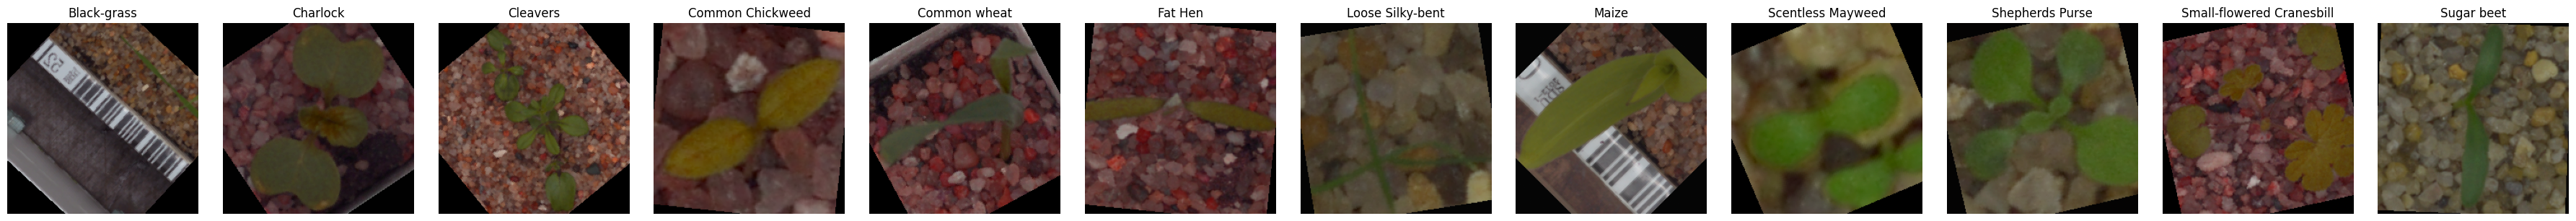
\includegraphics[width=0.9\linewidth]{../../resources/sample_images.png}}
    \caption{Sample images for each class in the dataset}
    \label{fig:sample-images}
\end{figure}

Fig.~\ref{fig:sample-images} shows one sample image for each class in the dataset, illustrating the different species. The images vary in background, lighting and growth stage, highlighting the challenges of visual similarity across species.

\subsection{Key Challenges}
Developing robust classification models for this task is not trivial. There are several challenges:

\begin{enumerate}
    \item \textbf{Inter-Class Similarity:} Certain seedlings can look strikingly similar, making it difficult for both humans and machines to distinguish between them.
    \item \textbf{Intra-Class Variability:} Even within a single species, seedlings can vary significantly in appearance due to differences in growth stage, lighting and background. This variability challenges models to learn consistent features that generalize well.
    \item \textbf{Data Limitations:} With approximately \textit{960} unique plants, the dataset could be considered modest for training deep learning models from scratch. While data augmentation can help to some extent, the relatively small dataset may still limit the complexity of models that can be effectively trained without overfitting.
    \item \textbf{Model Architecture Complexity:} Choosing the right model architecture, whether a custom CNN trained from scratch or a pre-trained deep CNN / Vision Transformer~(ViT), to learn complex visual features. Deeper models can capture more nuanced differences, but they can also be harder to train and require careful regularization to prevent overfitting.
\end{enumerate}

By clearly understanding these challenges and the broader context, model architectures can be proposed that address these difficulties. The following chapters discuss the strategies for model design, training optimization, model evaluation and analysis of results, ultimately leading to the approach that best addresses the core challenge of differentiating between plant seedling species. Finally, the conclusion summarizes the key findings and suggests potential areas for future research.